\section{Músicas e Efeitos Sonoros/Trilha Sonora}

\subsection{Introdução ao tema}
A trilha sonora  é composta por todos os áudios presentes no aplicativo, 
tais como músicas (de menus ou de background), efeitos especiais, vozes 
e efeitos de personagens e narrações - quando houver necessidade.

A proposta da trilha sonora é criar ambiência, de modo a melhorar a imersão
 no jogo e garantir feedback mais eficiente e claro das ações tomadas pelo
 personagem (controlado pelo jogador), ações de inimigos, estímulos,
 obstáculos e NPCs
\footnote{Non-player character (Personagem não jogável) - compreende um 
personagem que não pode ser controlado pelo jogador, embora possa fazer
 parte da ação do jogo.}. 
A trilha sonora deve ainda valorizar o uso do software, de modo a permitir
 novas possibilidades de interação e comunicação com o usuário, indo além
 das informações visuais que não atenderiam ao uso do mesmo ou o tornaria
 seu uso menos interativo, mais lento e cansativo.

A narração é um componente da trilha sonora que deve ser produzido de forma
 cuidadosa, principalmente em jogos direcionados para público infantil ou
 em processo de alfabetização, pois guiará as ações do jogador e permitirá
 uma ação mais rápida e efetiva em caso de dúvidas ou orientações quanto
 ao jogo.

A produção da trilha sonora pode ocorrer de três maneiras:
\begin{itemize}
\item Captação do áudio da voz humana, de instrumentos musicais ou de
 objetos sonoros
\footnote{Compreendem objetos, que não são necessariamente instrumentos
 musicais, mas que emitem sons que podem ser aproveitados em criações
 artísticas e musicais. São elementos de criação estudados por diversos 
compositores, destacando-se Pierre Henri Marie Schaeffer.}, 
através de gravadores digitais ou computadores conectados com outros
 periféricos, como placa de som, microfones e mesas de som, utilizando-se
 de softwares específicos para isso: Sound Forge, Audacity, Sonar entre 
outros disponíveis no mercado. O resultado obtido normalmente é um 
arquivo de áudio.
\item Produção através de recursos MIDI
\footnote{Musical Instrument Digital Interface - compreende uma interface
 de comunicação entre dispositivos que se utilizem deste protocolo. 
Estes dispositivos podem ser computadores, instrumentos musicais e 
placas de som.}
, uma estrutura de dados, ou seja, não compreendendo áudios. Estes 
dados funcionam como uma ``partitura'' que o computador consegue
 entender através de softwares específicos, como o Sonar e o Reason. 
Obtém-se como resultado, arquivos de dados com a extensão ``mid''.
\item Os programas citados conseguem ``tocar'' esta ``partitura'' e 
gerar um arquivo de áudio, através da ligação pela interface MIDI, com 
bancos de sons instalados no computador, ou em instrumentos que se 
utilizem desta estrutura. Essas ``partituras'' podem ser criadas e 
editadas em programas de edição musical com o Sibelius, Finale, Encore
 e MuseScore.
\item Composições interativas e composições algorítmicas geradas por
 softwares específicos como o Pure Data ou o Max/MSP. Para este tipo 
de composição é possível utilizar linhas de programação, como por 
exemplo, a linguagem C, e também em tempo real. Neste caso, o áudio 
é gerado através de algoritmos inseridos e processados no computador.
\end{itemize}

É importante ressaltar que músicas prontas também podem ser utilizadas
 e alteradas, desde que as autorizações pertinentes sejam obtidas ou 
que não sejam protegidas por Leis de Direitos Autorais
\footnote{Artigo 41 da Lei nº 9.610/98: relata que os direitos autorais 
perduram por setenta anos, a partir de 1º de janeiro do ano subsequente
 ao falecimento do compositor. Muitos outros artigos compreendem leis 
que devem ser de conhecimento do produtor musical.}. 

Este trabalho de produção pode ser elaborado em um software multipista,
 como o Cakewalk Sonar, que permite manipular simultaneamente informação
 MIDI e áudio. Na captura de tela da Figura \ref{img:midi}, retirada de
 Jesus (2008), observa-se as trilhas ou tracks, nas cores rosa escuro
 (bateria), amarelo (baixo), azul (percussão) e ciano (hammond) que
 compreendem informações MIDI (sinalizada como), indicada pelos traços
 que representam a ``partitura'' para o computador. Já a trilha em cinza 
escuro (guitarra) é composta por um áudio (sinalizado por ) proveniente
 de captação em linha, ou seja, com o instrumento conectado em uma mesa
 ou placa de som ou da captação realizada através de microfone. 

\begin{figure}[!ht]
 \centering
 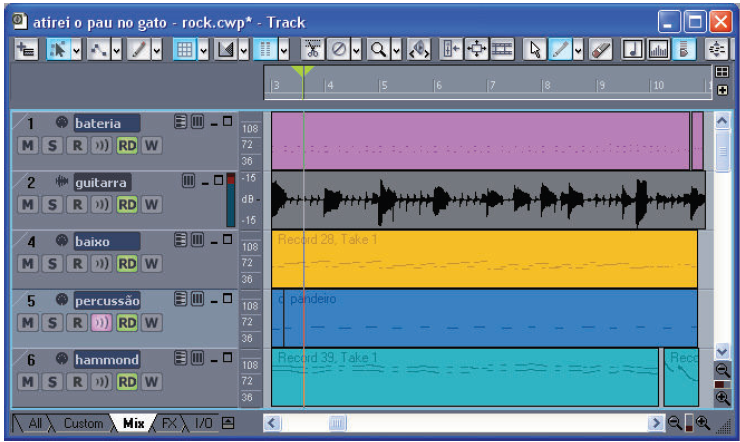
\includegraphics[scale=0.8]{musica_midi.png}
 \caption{Captura de tela demonstra as trilhas de áudio e MIDI. \cite{bib:musica_jesus}}
 \label{img:midi}
\end{figure}

A vantagem do uso de um software com estas características reside na
 rapidez da produção e na possibilidade de ouvir o resultado a ser 
obtido durante o processo, sem necessidade de finalizar o MIDI e o 
áudio em separado.
Outro software que apresenta como característica a produção musical
 estruturada em recursos MIDI e em áudio, é o Reason, da Empresa
 Propellerhead, que permite a conexão de instrumentos MIDI, gravando-os
 diretamente, ou importando arquivos ``.mid'' previamente elaborados em 
editores de partituras. Com o arquivo ``aberto'' dentro do Reason é
 possível alterá-lo ou acrescentar efeitos, como reverb
\footnote{Efeito que simula a reverberação do som em ambientes diversos.}
, chorus
\footnote{Efeito que simula a sensação de aumento das fontes sonoras.}
, flanger
\footnote{Efeito simular ao chorus, embora soando como se houvessem
 interferências no áudio.} 
e alterar o timbre
\footnote{Timbre corresponde à qualidade do som que nos permite
 identificar um instrumento, por exemplo, timbre do violão ou timbre 
da flauta.}
, ou seja, a qualidade do som a ser ouvida. Observa-se uma imagem do 
rack do Reason, com  uma ``prateleira'' e equipamentos virtuais, na 
Figura \ref{img:reason}.

\begin{figure}[!ht]
 \centering
 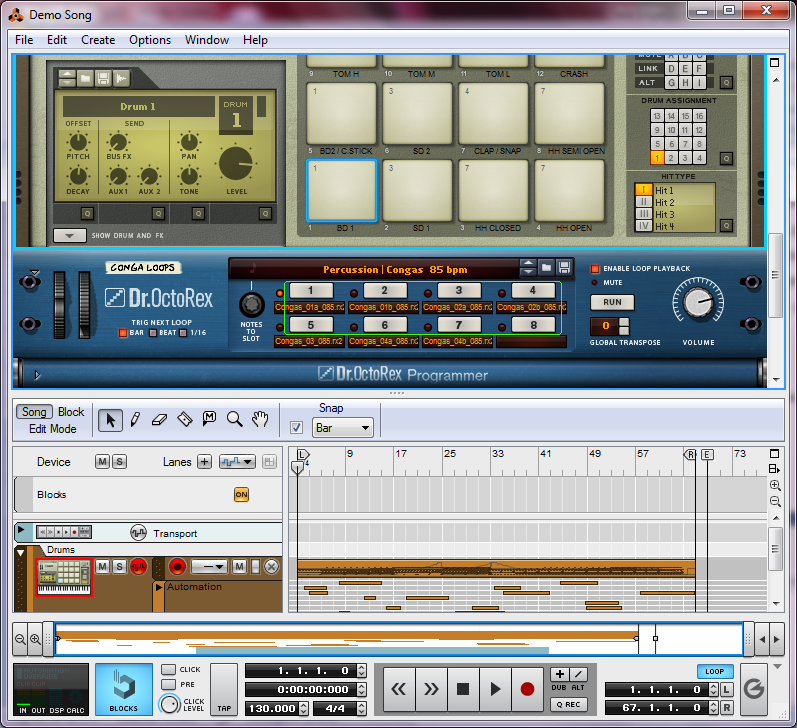
\includegraphics[scale=0.6]{musica_reason.png}
 \caption{Captura de tela do software Reason}
 \label{img:reason}
\end{figure}

Este software faz ainda o uso de refills ou banco de sons, permitindo 
a utilização de sons sampleados
\footnote{Trechos ou amostras de timbres de instrumentos musicais 
gravados previamente.}
 de alta fidelidade, tornando o som MIDI, desde que bem estruturado,
 praticamente equiparável ao de gravações de instrumentos reais. Samples 
ou amostras com resolução de 16 ou 24 bits são necessárias para se obter
 esta qualidade, bem como amostragem de 44.100 Hertz ou superior. 
A produção do áudio pode ser ainda incrementada utilizando-se recursos
de um game engine como o Unity, que permite tornar efeitos sonoros mais
 realistas. Um exemplo possível ocorre quando o personagem se aproxima 
de uma fonte sonora, como o fogo, neste momento a intensidade sonora
 aumentará.

\subsection{Propostas de sonorização para o jogo ``As crônicas 
de Medrash''}

\subsubsection{Efeitos sonoros}
Os efeitos sonoros que serão incluídos no jogo apresentam quatro
 funcionalidades, sendo elas:
\begin{itemize}
\item Sons de inimigos, que correspondem a cobra, urso, jacaré, abelha e tigre. 
Para a geração destes áudios serão feitos testes para que o resultado 
seja próximo ao som original dos animais, ou seja, mais realísticos. 
Faremos experimentos com busca em bancos de sons free e também a 
gravação através de objetos sonoros. 

\begin{itemize}
\item Cobra.
\begin{itemize}
\subitem Deslocamento: Som ativado no momento que a cobra se esta 
movimentando na terra, a cobra está patrulhando aleatoriamente no cenário.
\subitem Alerta da cobra: Som ativado quando a cobra fica no estado de alerta 
para atacar ao personagem.
\subitem Ataque da cobra:Som ativado no momento que a cobra ataca 
ao personagem 
\subitem Morte da cobra: Som ativado quando a cobra morre. 
\end{itemize}

\begin{itemize}
\item Urso.
\subitem Deslocamento: Som ativado no momento que ao urso se esta movimentando, 
o urso está patrulhando aleatoriamente no cenário.
\subitem Perseguição: Som ativado quando o urso persegue para atacar ao personagem.
\subitem Ataque do urso: Som ativado no momento que o urso ataca ao personagem, 
sons de rugido e de garra
\subitem Defensa do urso: Som ativado quando o urso se defende  
\subitem Morte do urso: Som ativado quando o urso morre.
\end{itemize}

\begin{itemize}
\item Jacaré.
\subitem Deslocamento: Som ativado no momento que o jacaré se esta movimentando, 
o jacaré está patrulhando aleatoriamente no cenário.
\subitem Perseguição: Som ativado quando o jacaré persegue para atacar ao personagem.
\subitem Ataque do jacaré: Som ativado no momento que o jacaré ataca ao personagem.
\subitem Morte do jacaré: Som ativado quando o jacaré morre.
\end{itemize}

\begin{itemize}
\item Enxame de Abelhas.
\subitem Deslocamento do enxame: Som ativado no momento que as abelhas estão 
no exame.
\subitem Perseguição: Som ativado quando as abelhas perseguem para atacar 
ao personagem.
\subitem Ataque do enxame: Som ativado no momento as abelhas ataca ao personagem
\end{itemize}

\begin{itemize}
\item Tigre.
\subitem Inicio: Somdo tigre corre afastado do personagem. 
\subitem Deslocamento: Som ativado no momento que o tigre se esta movimentando, 
o tigre está patrulhando aleatoriamente no cenário.
\subitem Perseguição: Som ativado quando o tigre persegue para atacar 
ao personagem.
\subitem Ataque: Som ativado no momento que o tigre ataca ao personagem, 
sons de saltos, rugidos e garras  
\subitem Cansado: Som ativado quando o tigre esta cansado.
\subitem Morte do tigre: Som ativado quando o tigre morre.
\end{itemize}



\end{itemize}

\item Sons do personagem Medrash, que incluirão sons correspondentes
 aos seus movimentos e ações: passos, saltar, pegar e atacar. A
 produção ocorre de forma idêntica à indicada nos sons dos inimigos.

\begin{itemize}
\item Medrash.
\subitem Passos na agua: som ativado no momento que o Medrash atravesse o rio 
que tem na fase 1. 
\subitem Passos na terra: som ativado ao momento que Medras se este movimentando 
atravessando a fase 
\subitem Saltos: som ativado no momento que o Medrash pula no transcurso da fase
\subitem Pegar: Som ativado quando o Medrash pega a comida para alimentar-se
\subitem Atacar: Som ativado quando ataca aos inimigos da fase
\subitem Morte do Medrash: som ativado quando acaba a barra de vida, 
ou seja, o Medrash morre
\end{itemize}

\item Sons do ambiente, os quais incluirão diferentes tipos de sons para os
principais elementos que compõem o cenário:
\begin{itemize}
\subitem Som do ar: som ativado para extinguir a chama da tocha. 
\subitem Som dos pássaros nas arvores: som ativado em alguns lugares da floresta 
do jogo 
\subitem Som da agua do rio: Este é ativado ao momento que o personagem chega 
perto do rio na primeira fase.
\subitem Som de pedras caindo: este som é ativado no momento que o personagem 
começa a trilha da primeira fase é se encontra como o primeiro objetivo do 
nível que é descer uma montanha pulando pedras as quais vai caído.
\subitem Som de fogo: este som  é ativado ao momento de que o personagem 
acenda a tocha.
\end{itemize}

\item Efeitos de menus, de forma a indicar que foi trocada uma opção no 
menu e que um item foi selecionado. Um som da ação do jogo poderá ser
 utilizado para tal função, possivelmente o som do ataque.
\end{itemize}

\subsubsection{Música para menus}
Compreende uma trilha de áudio com uma música que será apresentada toda
 vez que os menus forem carregados. Serão feitos testes para esta produção, 
verificando a viabilidade do uso de produção através de instrumentos
 acústicos ou MIDI. Como outro recurso poderão ser obtidos áudios já
 elaborados, sem direitos autorais, que permitam integração ao jogo.

\subsubsection{Músicas de background}
As músicas de background compreendem trilhas de áudio que possivelmente
 estarão presentes no momento da ação do jogo. As trilhas de áudio 
deverão compor a atmosfera do jogo, oferecendo características de 
cada fase. Isto deve oferecer maior imersão o jogador.

Assim como nas músicas para menus, a produção iniciará com testes, de 
forma a optar pelo melhor resultado, através de gravação em linha,
 utilização de recursos MIDI ou áudios preelaborados.
